\section{Methodology: Design of the Regime-Detection and Network-Learning Pipeline}
\label{sec:methodology-design}

This section merges the three design responsibilities of the team (data
and indicator pipeline; the regime-detection process and its internals;
Bayesian-network training and validation) into one coherent narrative,
since in practice none of the three can be designed independently of the
other two: the indicator pipeline's discretization choices determine
what the Bayesian network can possibly learn, and the regime-detection
process is itself one specific instance of that discretization.

\subsection{Data and Indicator Pipeline}
\label{sec:data-indicator-pipeline}

The GWP1 cleaning pipeline (the "Data Cleaning" section of that
report) produces 24 continuous, cleaned series at their native
frequency (daily for the 5 financial series, monthly for the 19
macroeconomic/geopolitical series). A Bayesian network, as implemented
by \texttt{pgmpy}, requires every node's domain to be a small, finite set
of categories -- a continuous price level or an unbounded percentage
change cannot be used directly. The indicator pipeline therefore has to
solve two distinct discretization problems, which we deliberately treat
differently because they are economically different problems:

\begin{enumerate}
  \item \textbf{The two headline price series (WTI, Brent).} Here the
    object of interest is not simply "high" or "low" values of the
    series (a price level has no natural absolute threshold -- WTI at
    \$80 might be a crash relative to a \$120 regime, or a rally
    relative to a \$40 regime), but the \emph{regime} generating the
    day-to-day fluctuations. This is precisely the problem a Hidden
    Markov Model is designed to solve, and is described in full in
    Section~\ref{sec:regime-process}.
  \item \textbf{The remaining 22 macroeconomic/geopolitical series.} For
    these, we are not trying to detect a persistent latent regime (most
    of the series, e.g.\ OPEC spare capacity, do not exhibit the kind of
    volatility clustering that motivates an HMM); instead the goal is
    simply to compare each series' period-over-period movement on a
    common, discrete scale. We compute the month-over-month percentage
    change of each series and discretize it into terciles (\emph{low},
    \emph{medium}, \emph{high}) via empirical quantiles
    (\texttt{pandas.qcut}). Terciles were chosen over a finer binning
    (e.g.\ quintiles) deliberately: with only 166 usable months of
    overlapping history (the panel is left-truncated to Brent's 2007
    start date, the shortest-history series in the group), a finer
    discretization would leave too few observations per bin for
    Hill-Climbing's internal BIC score to distinguish genuine structure
    from sampling noise.
\end{enumerate}

Both discretization paths converge on the same final artifact: a single
\texttt{pandas.DataFrame} of 24 categorical columns at monthly
frequency, 166 rows, which is the only input the Bayesian-network stage
(Section~\ref{sec:bn-training-validation}) ever sees. This separation of
concerns -- discretize once, learn structure on the discretized panel --
is what keeps the two models composable: either one can be swapped out
(e.g.\ a different regime-detection scheme, or a finer/coarser
discretization) without touching the other.

\subsection{The Regime-Detection Process and HMM Internals}
\label{sec:regime-process}

For each of the two headline series, the pipeline:

\begin{enumerate}
  \item \textbf{Transforms} the cleaned daily price series into daily
    log returns, $r_t = \log(P_t) - \log(P_{t-1})$. Log returns, not
    levels, are the input to the HMM for the same reason regressions are
    typically run on returns rather than levels: returns are
    approximately stationary (constant unconditional mean/variance over
    the full sample), which is required for the fitted per-state
    Gaussian emission parameters to be meaningfully comparable across
    the whole 2000--2026 (WTI) / 2007--2026 (Brent) history, rather than
    reflecting one period's price scale.
  \item \textbf{Trains} a 3-state \texttt{HiddenMarkovRegimeModel} via
    Baum-Welch (Section~\ref{sec:algorithms}; treated as a black box
    here, having already been validated in isolation on the toy
    example). $K=3$ states is a deliberate modelling choice, not a
    free hyperparameter tuned on this data: it is chosen to match the
    team's three qualitative labels (bear/stagnant/bull), mirroring
    Alvi's original three-regime framing, rather than selected by
    maximizing a likelihood or information criterion over $K$, which
    would risk simply fitting more, less-interpretable states to noise.
  \item \textbf{Decodes} the single most likely state path for the
    entire history via Viterbi (again a black box at this stage),
    producing one of $\{0, 1, 2\}$ per trading day.
  \item \textbf{Assigns latent meaning} to each of the three arbitrary
    state indices by ranking the fitted emission means
    $\hat\mu_0,\hat\mu_1,\hat\mu_2$: the lowest-mean state is labelled
    \emph{bear}, the middle \emph{stagnant}, and the highest \emph{bull}
    (\texttt{oilbn.models.hmm.\allowbreak label\_states\_by\_mean}). This is a
    necessary step because Baum-Welch (like all EM algorithms) has no
    notion of state \emph{identity} -- state "0" is an arbitrary index
    assigned at initialization, not inherently "the bear state" --, so
    the economically meaningful label has to be attached after fitting,
    by inspecting the fitted parameters.
\end{enumerate}

Table~\ref{tab:regime-durations} reports the resulting regime
statistics. Two findings validate the model qualitatively before it is
ever used downstream: first, decoded bear spells are short and sharp
(WTI: mean 21.5 trading days) while bull spells are long and gradual
(WTI: mean 140.7 days) -- exactly the asymmetric "sharp crash, slow
recovery" pattern visible by eye in Figure~\ref{fig:wti-regimes} and
consistent with the volatility-clustering stylized fact established in
GWP1. Second, the well-known 2008--09, 2014--16, and 2020 oil-price
collapses are each correctly flagged as (part of) a bear spell by the
unsupervised decoding, without the model ever being told when those
events occurred.

\begin{table}[H]
  \centering
  \caption{Decoded regime-spell durations (trading days).}
  \label{tab:regime-durations}
  \begin{tabular}{lrrrrr}
    \toprule
    & \multicolumn{2}{c}{WTI} & \multicolumn{2}{c}{Brent} & \\
    Regime & Count & Mean & Count & Mean & \\
    \midrule
    Bear     & 13 & 21.5  & 13 & 27.8 & \\
    Stagnant & 36 & 84.4  & 37 & 64.8 & \\
    Bull     & 23 & 140.7 & 24 & 83.9 & \\
    \bottomrule
  \end{tabular}
\end{table}

\begin{figure}[H]
  \centering
  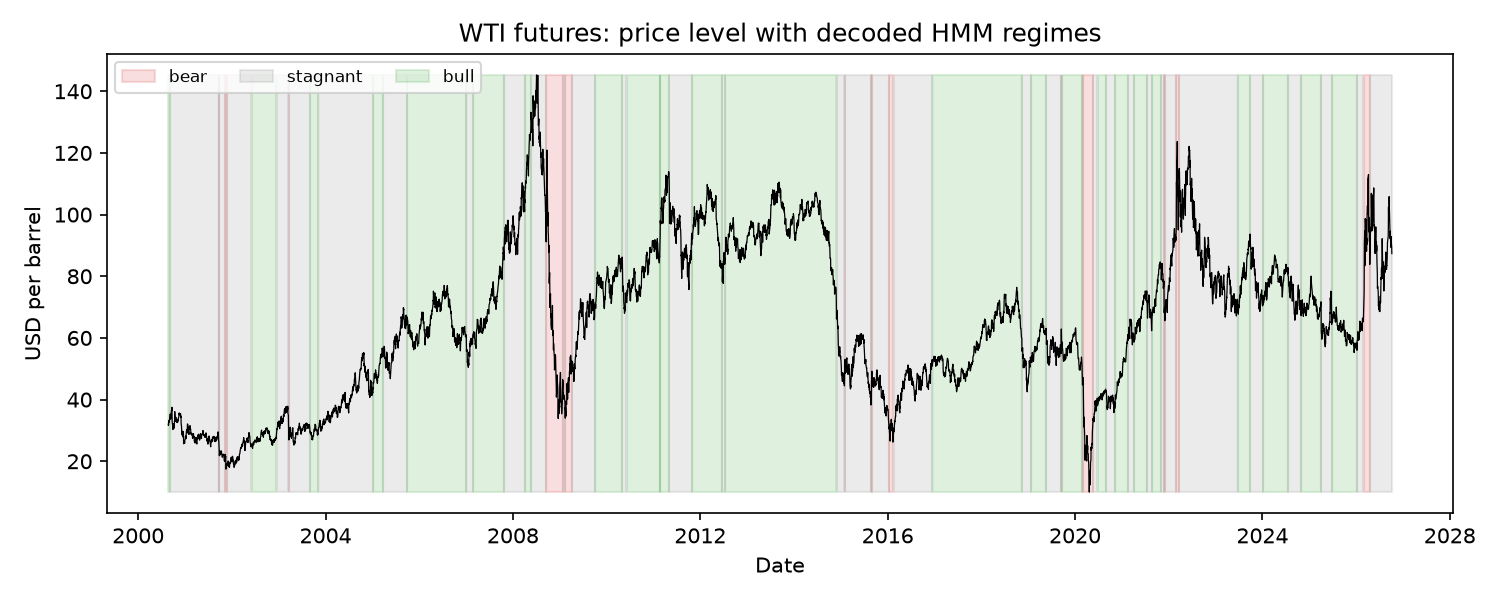
\includegraphics[width=\textwidth]{figures/wti_regimes.png}
  \caption{WTI futures price level shaded by decoded HMM regime.}
  \label{fig:wti-regimes}
\end{figure}

Finally, the daily regime labels are resampled to month-end frequency by
taking the modal (most frequently occurring) regime within each month,
so they can be merged with the inherently-monthly macroeconomic and
geopolitical series into the single discrete panel described in
Section~\ref{sec:data-indicator-pipeline}.

\subsection{Bayesian-Network Training and Validation}
\label{sec:bn-training-validation}

With the 24-column discrete monthly panel in hand, structure learning
and parameter learning proceed exactly as described in the GWP1 report
(Sections 4--5 of that report): \texttt{OilPriceBayesianNetwork} wraps
\texttt{pgmpy}'s \texttt{HillClimbSearch} (BIC score, \texttt{"bic-d"})
for the structure, and a Bayesian/BDeu-prior estimator for the CPDs. Two
design decisions are specific to this stage and are documented here:

\begin{description}
  \item[\texttt{max\_indegree=3}.] With only 166 monthly observations
    across 24 variables, allowing nodes an unbounded number of parents
    would let Hill-Climbing fit an overly dense graph whose CPDs are
    estimated from only a handful of observations per parent-value
    combination -- the same small-sample risk flagged for parameter
    learning in the GWP1 report, here addressed structurally rather than
    only through the estimator's prior.
  \item[Bayesian (BDeu) over Maximum-Likelihood parameter estimation.]
    Both are implemented and exposed via \texttt{fit\_parameters(...,
    estimator=...)}; we use the Bayesian estimator as the default for
    exactly the reason given in the GWP1 report's parameter-learning
    discussion -- several parent-value combinations in a 166-row,
    many-parent CPD are observed only once or twice, and an
    uninformative BDeu prior (equivalent sample size 5) regularizes
    those combinations' probabilities away from the harsh 0/1 extremes
    that pure relative-frequency (MLE) estimation would otherwise
    assign them.
\end{description}

\textbf{Training/validation rationale.} Because this panel is a single
chronologically-ordered time series (not i.i.d.\ cross-sectional data),
a random train/validation split would leak information from the future
into the training set and understate how much the learned structure
would actually generalize to genuinely new, later data. We therefore use
a chronological 80/20 split (training: 2007-07 to 2018-06, 132 months;
validation: 2018-07 to 2021-04, 34 months) purely as a \emph{structural
stability} check at this stage: Hill-Climbing is re-run on the training
subset alone, and its learned edge set is compared against the
full-sample edge set. 14 of the 15 full-sample edges (93\%) are also
recovered from the training subset alone, which is reassuring evidence
that the learned structure reflects a genuine, stable feature of the
underlying data-generating process rather than an artifact of the
specific 166-month sample used. The formal train/validation/test
harness with forecast-accuracy metrics (\texttt{DatasetSplitter},
\texttt{ForecastEvaluator}) is built in GWP3, once the full modelling
pipeline (this report) is finalized.

Figure~\ref{fig:bn-structure} shows the full learned network. Several
edges are directly interpretable and economically sensible: the
upstream link \texttt{brent\_regime} $\to$ \texttt{wti\_regime} (the two benchmark
crudes move together, consistent with the GWP1 correlation heatmap's
$0.98$ level correlation between them); a direct link between
\texttt{cpi\_energy\_chg} and \texttt{ppi\_oil\_gas\_extraction\_chg}
(the consumer energy price index and the upstream oil \& gas producer
price index move together, as expected for two measures of the same
underlying price pass-through); and the OPEC capacity chain
\texttt{opec\_production\_capacity\_chg} $\to$ \texttt{supply\_opec\_chg} $\to$
\texttt{opec\_spare\_capacity\_chg}, which mirrors the accounting identity
"spare capacity = production capacity $-$ actual production" almost
exactly. The Markov blanket of \texttt{wti\_regime} -- the minimal set
of variables that screens it off from the rest of the network
(the "Markov Chains, Hidden Markov Models, and the Markov Blanket"
section of the GWP1 report) -- is
$\{\texttt{brent\_regime}, \texttt{capacity\_oil\_gas\_extraction\_chg},
\texttt{indprod\_oil\_gas\_support\_chg}\}$, and conditioning on the
first of these alone already produces a sharp posterior shift: $P(\text{wti
bull} \mid \text{brent bull}) = 0.973$ versus $P(\text{wti bear} \mid
\text{brent bear}) = 0.846$, both far from the roughly-uniform
unconditional regime frequencies.

One honest caveat on reproducibility: Hill-Climbing with a BIC score can
assign \emph{identical} scores to two different orientations of the same
edge when the underlying variables are only weakly directionally
identifiable from observational data alone (a known property of
score-equivalent Markov-equivalence classes). In practice this means a
handful of edge \emph{directions} (e.g.\ \texttt{usd\_index\_chg} $\to$
\texttt{sp500\_chg} versus the reverse) can flip between runs depending
on tie-breaking order, even though the \emph{skeleton} (which pairs of
variables are connected at all) and the Markov blanket of the two
regime nodes are stable across runs -- exactly the property verified by
the training/validation check above.

\begin{figure}[H]
  \centering
  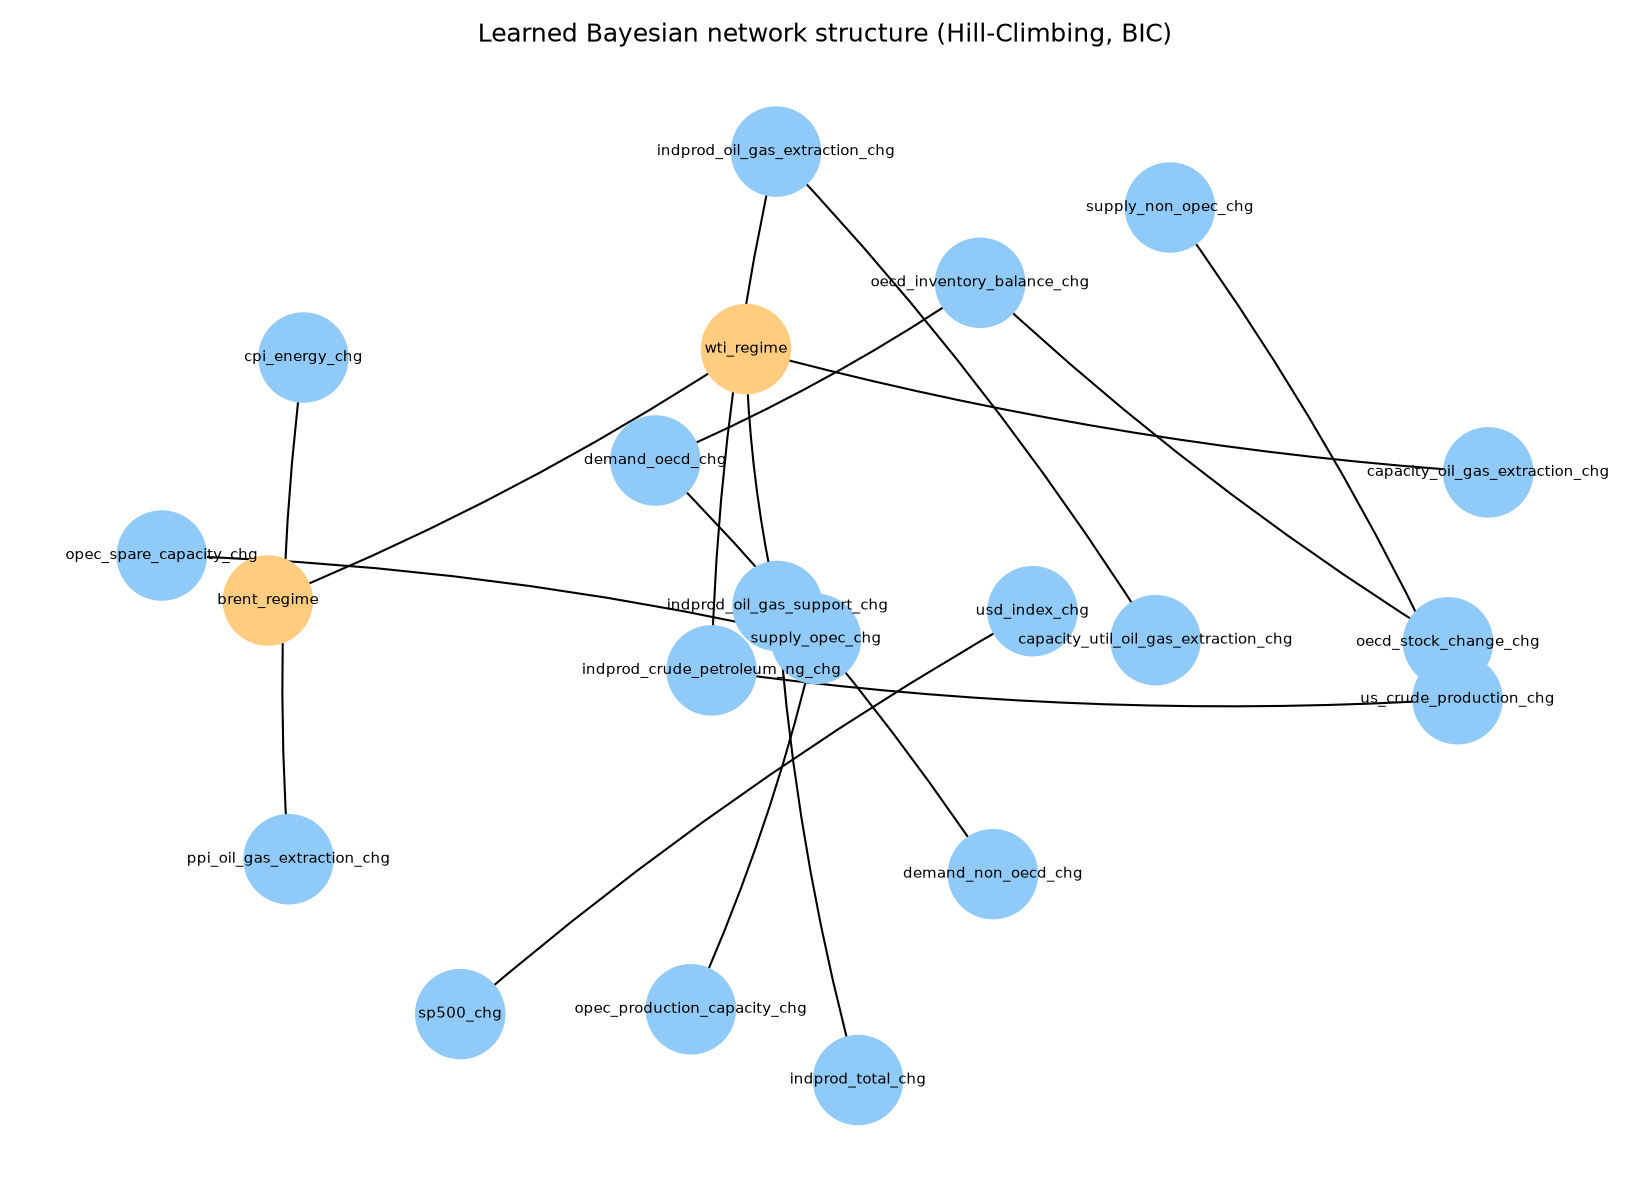
\includegraphics[width=\textwidth]{figures/bayesian_network_structure.png}
  \caption{Learned Bayesian-network structure (Hill-Climbing, BIC score,
    max in-degree 3) over the 24-variable discrete monthly panel.}
  \label{fig:bn-structure}
\end{figure}
